\PassOptionsToPackage{unicode=true}{hyperref} % options for packages loaded elsewhere
\PassOptionsToPackage{hyphens}{url}
%
\documentclass[10pt,xcolor=table,color={dvipsnames,usenames},ignorenonframetext,usepdftitle=false,french]{beamer}
\setbeamertemplate{caption}[numbered]
\setbeamertemplate{caption label separator}{: }
\setbeamercolor{caption name}{fg=normal text.fg}
\beamertemplatenavigationsymbolsempty
\usepackage{caption}
\captionsetup{skip=0pt,belowskip=0pt}
%\setlength\abovecaptionskip{-15pt}
\usepackage{lmodern}
\usepackage{amssymb,amsmath,mathtools,multirow}
\usepackage{float,hhline}
\usepackage{tikz,pgfplots}
\usepackage[tikz]{bclogo}
\usepackage{ifxetex,ifluatex}
\usepackage{fixltx2e} % provides \textsubscript
\ifnum 0\ifxetex 1\fi\ifluatex 1\fi=0 % if pdftex
  \usepackage[T1]{fontenc}
  \usepackage[utf8]{inputenc}
  \usepackage{textcomp} % provides euro and other symbols
\else % if luatex or xelatex
  \usepackage{unicode-math}
  \defaultfontfeatures{Ligatures=TeX,Scale=MatchLowercase}
\fi
\usetheme[coding=utf8,language=french,
,titlepagelogo=img/logoinsee
,secondlogo=true
]{TorinoTh}
\titlepagesecondlogo{img/BCEAO}
% use upquote if available, for straight quotes in verbatim environments
\IfFileExists{upquote.sty}{\usepackage{upquote}}{}
% use microtype if available
\IfFileExists{microtype.sty}{%
\usepackage[]{microtype}
\UseMicrotypeSet[protrusion]{basicmath} % disable protrusion for tt fonts
}{}
\IfFileExists{parskip.sty}{%
\usepackage{parskip}
}{% else
\setlength{\parindent}{0pt}
\setlength{\parskip}{6pt plus 2pt minus 1pt}
}
\usepackage{hyperref}
\hypersetup{
            pdftitle={1 - R et JDemetra+},
            pdfauthor={Dominique Ladiray et Alain Quartier-la-Tente},
            pdfborder={0 0 0},
            breaklinks=true}
\urlstyle{same}  % don't use monospace font for urls
\newif\ifbibliography
\usepackage{color}
\usepackage{fancyvrb}
\newcommand{\VerbBar}{|}
\newcommand{\VERB}{\Verb[commandchars=\\\{\}]}
\DefineVerbatimEnvironment{Highlighting}{Verbatim}{commandchars=\\\{\}}
% Add ',fontsize=\small' for more characters per line
\usepackage{framed}
\definecolor{shadecolor}{RGB}{248,248,248}
\newenvironment{Shaded}{\begin{snugshade}}{\end{snugshade}}
\newcommand{\AlertTok}[1]{\textcolor[rgb]{0.94,0.16,0.16}{#1}}
\newcommand{\AnnotationTok}[1]{\textcolor[rgb]{0.56,0.35,0.01}{\textbf{\textit{#1}}}}
\newcommand{\AttributeTok}[1]{\textcolor[rgb]{0.77,0.63,0.00}{#1}}
\newcommand{\BaseNTok}[1]{\textcolor[rgb]{0.00,0.00,0.81}{#1}}
\newcommand{\BuiltInTok}[1]{#1}
\newcommand{\CharTok}[1]{\textcolor[rgb]{0.31,0.60,0.02}{#1}}
\newcommand{\CommentTok}[1]{\textcolor[rgb]{0.56,0.35,0.01}{\textit{#1}}}
\newcommand{\CommentVarTok}[1]{\textcolor[rgb]{0.56,0.35,0.01}{\textbf{\textit{#1}}}}
\newcommand{\ConstantTok}[1]{\textcolor[rgb]{0.00,0.00,0.00}{#1}}
\newcommand{\ControlFlowTok}[1]{\textcolor[rgb]{0.13,0.29,0.53}{\textbf{#1}}}
\newcommand{\DataTypeTok}[1]{\textcolor[rgb]{0.13,0.29,0.53}{#1}}
\newcommand{\DecValTok}[1]{\textcolor[rgb]{0.00,0.00,0.81}{#1}}
\newcommand{\DocumentationTok}[1]{\textcolor[rgb]{0.56,0.35,0.01}{\textbf{\textit{#1}}}}
\newcommand{\ErrorTok}[1]{\textcolor[rgb]{0.64,0.00,0.00}{\textbf{#1}}}
\newcommand{\ExtensionTok}[1]{#1}
\newcommand{\FloatTok}[1]{\textcolor[rgb]{0.00,0.00,0.81}{#1}}
\newcommand{\FunctionTok}[1]{\textcolor[rgb]{0.00,0.00,0.00}{#1}}
\newcommand{\ImportTok}[1]{#1}
\newcommand{\InformationTok}[1]{\textcolor[rgb]{0.56,0.35,0.01}{\textbf{\textit{#1}}}}
\newcommand{\KeywordTok}[1]{\textcolor[rgb]{0.13,0.29,0.53}{\textbf{#1}}}
\newcommand{\NormalTok}[1]{#1}
\newcommand{\OperatorTok}[1]{\textcolor[rgb]{0.81,0.36,0.00}{\textbf{#1}}}
\newcommand{\OtherTok}[1]{\textcolor[rgb]{0.56,0.35,0.01}{#1}}
\newcommand{\PreprocessorTok}[1]{\textcolor[rgb]{0.56,0.35,0.01}{\textit{#1}}}
\newcommand{\RegionMarkerTok}[1]{#1}
\newcommand{\SpecialCharTok}[1]{\textcolor[rgb]{0.00,0.00,0.00}{#1}}
\newcommand{\SpecialStringTok}[1]{\textcolor[rgb]{0.31,0.60,0.02}{#1}}
\newcommand{\StringTok}[1]{\textcolor[rgb]{0.31,0.60,0.02}{#1}}
\newcommand{\VariableTok}[1]{\textcolor[rgb]{0.00,0.00,0.00}{#1}}
\newcommand{\VerbatimStringTok}[1]{\textcolor[rgb]{0.31,0.60,0.02}{#1}}
\newcommand{\WarningTok}[1]{\textcolor[rgb]{0.56,0.35,0.01}{\textbf{\textit{#1}}}}
\usepackage{graphicx,grffile}
\makeatletter
\def\maxwidth{\ifdim\Gin@nat@width>\linewidth\linewidth\else\Gin@nat@width\fi}
\def\maxheight{\ifdim\Gin@nat@height>\textheight\textheight\else\Gin@nat@height\fi}
\makeatother
% Scale images if necessary, so that they will not overflow the page
% margins by default, and it is still possible to overwrite the defaults
% using explicit options in \includegraphics[width, height, ...]{}
\setkeys{Gin}{width=\maxwidth,height=\maxheight,keepaspectratio}
% Prevent slide breaks in the middle of a paragraph:
\widowpenalties 1 10000
\raggedbottom
\AtBeginPart{
  \let\insertpartnumber\relax
  \let\partname\relax
  \frame{\partpage}
}
\AtBeginSection{
  \ifbibliography
  \else
    \begin{frame}{Sommaire}
    \tableofcontents[currentsection, hideothersubsections]
    \end{frame}
  \fi
}
\setlength{\emergencystretch}{3em}  % prevent overfull lines
\providecommand{\tightlist}{%
  %\setlength{\itemsep}{0pt}
  \setlength{\parskip}{0pt}
  }
\setcounter{secnumdepth}{0}

% set default figure placement to htbp
\makeatletter
\def\fps@figure{htbp}
\makeatother

\usepackage{animate}
\usepackage{fontawesome5}

\title{1 - R et JDemetra+}
\ateneo{BCEAO - 20 au 25 janvier 2019}
\author{Dominique Ladiray et Alain Quartier-la-Tente}
\date{}


\setrellabel{}

\setcandidatelabel{}

\rel{}
\division{(\href{mailto:dominique.ladiray@insee.fr}{\nolinkurl{dominique.ladiray@insee.fr}}
et
\href{mailto:alain.quartier@yahoo.fr}{\nolinkurl{alain.quartier@yahoo.fr}})}

\departement{}

\DeclareMathOperator{\Cov}{Cov}
\newcommand{\E}[1]{\mathbb{E}\left[ #1 \right]}
\newcommand{\V}[1]{\mathbb{V}\left[ #1 \right]}
\newcommand{\cov}[2]{\Cov\left( #1\,,\,#2 \right)}

\begin{document}
\frame[plain,noframenumbering]{\titlepage}

\hypertarget{le-jwsacruncher}{%
\section{Le JWSACruncher}\label{le-jwsacruncher}}

\hypertarget{introduction}{%
\subsection{Introduction}\label{introduction}}

\begin{frame}{Le JWSACruncher}
\protect\hypertarget{le-jwsacruncher-1}{}

Objectifs du cruncher : mettre à jour un workspace de JDemetra+ et
exporter les résultats à partir de la console (en \emph{batch}), sans
devoir ouvrir JDemetra+ : très utile pour la production. Quelques liens
:

\begin{itemize}
\item
  pour télécharger le cruncher
  \url{https://github.com/jdemetra/jwsacruncher/releases}.
\item
  l'aide associée au cruncher
  \url{https://github.com/jdemetra/jwsacruncher/wiki}.
\item
  configuration du cruncher une version portable de Java :
  \url{https://github.com/AQLT/JDCruncheR/wiki/Installation-et-configuration-de-JDemetra--et-du-cruncher}.
\end{itemize}

\end{frame}

\begin{frame}{Le cruncher}
\protect\hypertarget{le-cruncher}{}

Pour lancer le cruncher de JDemetra+ il faut :

\begin{itemize}
\item
  le cruncher~;
\item
  un fichier contenant les paramètres sur la méthode de rafraîchissement
  à utilisée pour mettre à jour le workspace et sur les paramètres
  d'export~;
\item
  un workspace valide de JDemetra+.
\end{itemize}

\end{frame}

\hypertarget{lancement-du-cruncher-depuis-r}{%
\subsection{Lancement du cruncher depuis
R}\label{lancement-du-cruncher-depuis-r}}

\begin{frame}[fragile]{Installation du package}
\protect\hypertarget{installation-du-package}{}

Le package \texttt{rjwsacruncher} est une interface autour du
JWSACruncher.

Il est disponible sur le CRAN a une page GitHub associée :
\url{https://github.com/AQLT/rjwsacruncher}.

\begin{Shaded}
\begin{Highlighting}[]
\KeywordTok{install.packages}\NormalTok{(}\StringTok{"rjwsacruncher"}\NormalTok{)}
\end{Highlighting}
\end{Shaded}

\end{frame}

\begin{frame}[fragile]{Utilisation de rjwsacruncher (1/3)}
\protect\hypertarget{utilisation-de-rjwsacruncher-13}{}

Une vignette décrit plus précisément la procédure pour utiliser le
cruncher à partir du package :

\begin{Shaded}
\begin{Highlighting}[]
\KeywordTok{browseVignettes}\NormalTok{(}\StringTok{"rjwsacruncher"}\NormalTok{)}
\end{Highlighting}
\end{Shaded}

Pour charger le package :

\begin{Shaded}
\begin{Highlighting}[]
\KeywordTok{library}\NormalTok{(rjwsacruncher)}
\end{Highlighting}
\end{Shaded}

\end{frame}

\begin{frame}[fragile]{Utilisation de rjwsacruncher (2/3)}
\protect\hypertarget{utilisation-de-rjwsacruncher-23}{}

Trois options vont être utiles : \texttt{default\_matrix\_item}
(diagnostics à exporter), \texttt{default\_tsmatrix\_series} (séries
temporelles à exporter) et \texttt{cruncher\_bin\_directory} (chemin
vers le cruncher).

Pour afficher les valeurs :

\begin{Shaded}
\begin{Highlighting}[]
\KeywordTok{getOption}\NormalTok{(}\StringTok{"default_matrix_item"}\NormalTok{)}
\KeywordTok{getOption}\NormalTok{(}\StringTok{"default_tsmatrix_series"}\NormalTok{)}
\KeywordTok{getOption}\NormalTok{(}\StringTok{"cruncher_bin_directory"}\NormalTok{)}
\end{Highlighting}
\end{Shaded}

Utiliser la fonction \texttt{options()} pour les modifier. Par exemple :

\begin{Shaded}
\begin{Highlighting}[]
\KeywordTok{options}\NormalTok{(}\DataTypeTok{default_matrix_item =} \KeywordTok{c}\NormalTok{(}\StringTok{"likelihood.aic"}\NormalTok{,}
                                \StringTok{"likelihood.aicc"}\NormalTok{,}
                                \StringTok{"likelihood.bic"}\NormalTok{,}
                                \StringTok{"likelihood.bicc"}\NormalTok{))}
\KeywordTok{options}\NormalTok{(}\DataTypeTok{default_tsmatrix_series =} \KeywordTok{c}\NormalTok{(}\StringTok{"sa"}\NormalTok{, }\StringTok{"sa_f"}\NormalTok{))}
\KeywordTok{options}\NormalTok{(}\DataTypeTok{cruncher_bin_directory =}
            \StringTok{"Y:/Logiciels/jwsacruncher-2.2.0/jdemetra-cli-2.2.0/bin"}\NormalTok{)}
\end{Highlighting}
\end{Shaded}

\end{frame}

\begin{frame}[fragile]{Utilisation de rjwsacruncher (3/3)}
\protect\hypertarget{utilisation-de-rjwsacruncher-33}{}

Une fois les trois options précédentes validées le plus simple est
d'utiliser la fonction \texttt{cruncher\_and\_param()} :

\begin{Shaded}
\begin{Highlighting}[]
\KeywordTok{cruncher_and_param}\NormalTok{() }\CommentTok{# lancement avec paramètres par défaut}

\KeywordTok{cruncher_and_param}\NormalTok{(}\DataTypeTok{workspace =} \StringTok{"D:/Campagne_CVS/ipi.xml"}\NormalTok{,}
                   \DataTypeTok{policy =} \StringTok{"lastoutliers"}\NormalTok{)}
\end{Highlighting}
\end{Shaded}

Pour voir l'aide associée à une fonction, utiliser \texttt{help()} ou
\texttt{?} :

\begin{Shaded}
\begin{Highlighting}[]
\NormalTok{?cruncher_and_param}
\KeywordTok{help}\NormalTok{(cruncher_and_param)}
\end{Highlighting}
\end{Shaded}

\(\longrightarrow\) Dans le TP le cruncher sera lancé en créant un
fichier de paramètres

\end{frame}

\hypertarget{lancer-jdemetra-depuis-r}{%
\section{Lancer JDemetra+ depuis R}\label{lancer-jdemetra-depuis-r}}

\begin{frame}[fragile]{RJDemetra

\includegraphics[height = 1.5cm]{img/rjdemetra_logo.png}}
\protect\hypertarget{rjdemetra}{}

RJDemetra est un package qui permet de lancer les routines de JDemetra+
depuis R

\large\faGithub\normalsize : \url{https://github.com/jdemetra/rjdemetra}

Page web : \url{https://jdemetra.github.io/rjdemetra/}

Pour l'installer :

\begin{Shaded}
\begin{Highlighting}[]
\KeywordTok{install.packages}\NormalTok{(}\StringTok{"RJDemetra"}\NormalTok{)}
\end{Highlighting}
\end{Shaded}

\(\rightarrow\) Peut être utilisé pour développer de nouveaux outils
pour aider la production

\(\rightarrow\) Il faut Java 8 ou plus pour l'utiliser. En cas de
problème d'installation :
\url{https://github.com/jdemetra/rjdemetra/wiki/Installation-manual}

\end{frame}

\hypertarget{current-status}{%
\subsection{Current status}\label{current-status}}

\begin{frame}[fragile]{Current status}
\protect\hypertarget{current-status-1}{}

\begin{itemize}
\tightlist
\item
  RegARIMA, TRAMO-SEATS et X-13-ARIMA :

  \begin{itemize}
  \tightlist
  \item
    spécifications prédéfinies et personnalisées
  \item
    classes S3 avec des méthodes plot, summary, print
  \end{itemize}
\end{itemize}

\medskip

\begin{itemize}
\tightlist
\item
  Manipulation de workspaces JD+ :

  \begin{itemize}
  \tightlist
  \item
    Import de workspaces to avec le modèle CVS
  \item
    Export des modèles R créé par RJDemetra
  \end{itemize}
\end{itemize}

\medskip

\begin{itemize}
\tightlist
\item
  Contient une base de données (\texttt{ipi\_c\_eu}) : les IPI dans
  l'industrie manufacturière dans l'UE
\end{itemize}

\end{frame}

\hypertarget{regarima-exemples}{%
\subsection{RegARIMA : exemples}\label{regarima-exemples}}

\begin{frame}[fragile]{RegARIMA : exemples (1/4)}
\protect\hypertarget{regarima-exemples-14}{}

\begin{Shaded}
\begin{Highlighting}[]
\KeywordTok{library}\NormalTok{(RJDemetra)}
\NormalTok{ipch_benin <-}\StringTok{ }\NormalTok{ipch_benin[,}\StringTok{"ensemble"}\NormalTok{]}
\NormalTok{regarima_model <-}\StringTok{ }\KeywordTok{regarima_x13}\NormalTok{(ipch_benin, }\DataTypeTok{spec =} \StringTok{"RG4c"}\NormalTok{)}
\NormalTok{regarima_model}
\end{Highlighting}
\end{Shaded}

\begin{verbatim}
## y = regression model + arima (0, 1, 0, 0, 1, 1)
## Log-transformation: no
## Coefficients:
##           Estimate Std. Error
## BTheta(1)  -0.9145      0.036
## 
##             Estimate Std. Error
## LS (1-2012)    4.379      0.824
## AO (4-2015)   -2.747      0.587
## AO (6-2009)   -2.322      0.582
## 
## 
## Residual standard error: 0.8265 on 237 degrees of freedom
## Log likelihood =  -308, aic =   626 aicc = 626.3, bic(corrected for length) = -0.2903
\end{verbatim}

\end{frame}

\begin{frame}[fragile]{RegARIMA : exemples (2/4)}
\protect\hypertarget{regarima-exemples-24}{}

\footnotesize

\begin{Shaded}
\begin{Highlighting}[]
\KeywordTok{summary}\NormalTok{(regarima_model)}
\end{Highlighting}
\end{Shaded}

\begin{verbatim}
## y = regression model + arima (0, 1, 0, 0, 1, 1)
## 
## Model: RegARIMA - X13
## Estimation span: from 1-1997 to 3-2018
## Log-transformation: no
## Regression model: no mean, no trading days effect, no leap year effect, no Easter effect, outliers(3)
## 
## Coefficients:
## ARIMA: 
##           Estimate Std. Error T-stat Pr(>|t|)    
## BTheta(1)  -0.9145     0.0355 -25.76   <2e-16 ***
## ---
## Signif. codes:  0 '***' 0.001 '**' 0.01 '*' 0.05 '.' 0.1 ' ' 1
## 
## Regression model: 
##             Estimate Std. Error T-stat Pr(>|t|)    
## LS (1-2012)   4.3790     0.8241  5.314 2.43e-07 ***
## AO (4-2015)  -2.7470     0.5869 -4.681 4.76e-06 ***
## AO (6-2009)  -2.3224     0.5818 -3.992 8.71e-05 ***
## ---
## Signif. codes:  0 '***' 0.001 '**' 0.01 '*' 0.05 '.' 0.1 ' ' 1
## 
## 
## Residual standard error: 0.8265 on 237 degrees of freedom
## Log likelihood =  -308, aic =   626, aicc = 626.3, bic(corrected for length) = -0.2903
\end{verbatim}

\end{frame}

\begin{frame}[fragile]{RegARIMA : exemples (3/4)}
\protect\hypertarget{regarima-exemples-34}{}

\begin{Shaded}
\begin{Highlighting}[]
\KeywordTok{layout}\NormalTok{(}\KeywordTok{matrix}\NormalTok{(}\DecValTok{1}\OperatorTok{:}\DecValTok{6}\NormalTok{, }\DecValTok{3}\NormalTok{, }\DecValTok{2}\NormalTok{));}\KeywordTok{plot}\NormalTok{(regarima_model, }\DataTypeTok{ask =} \OtherTok{FALSE}\NormalTok{)}
\end{Highlighting}
\end{Shaded}

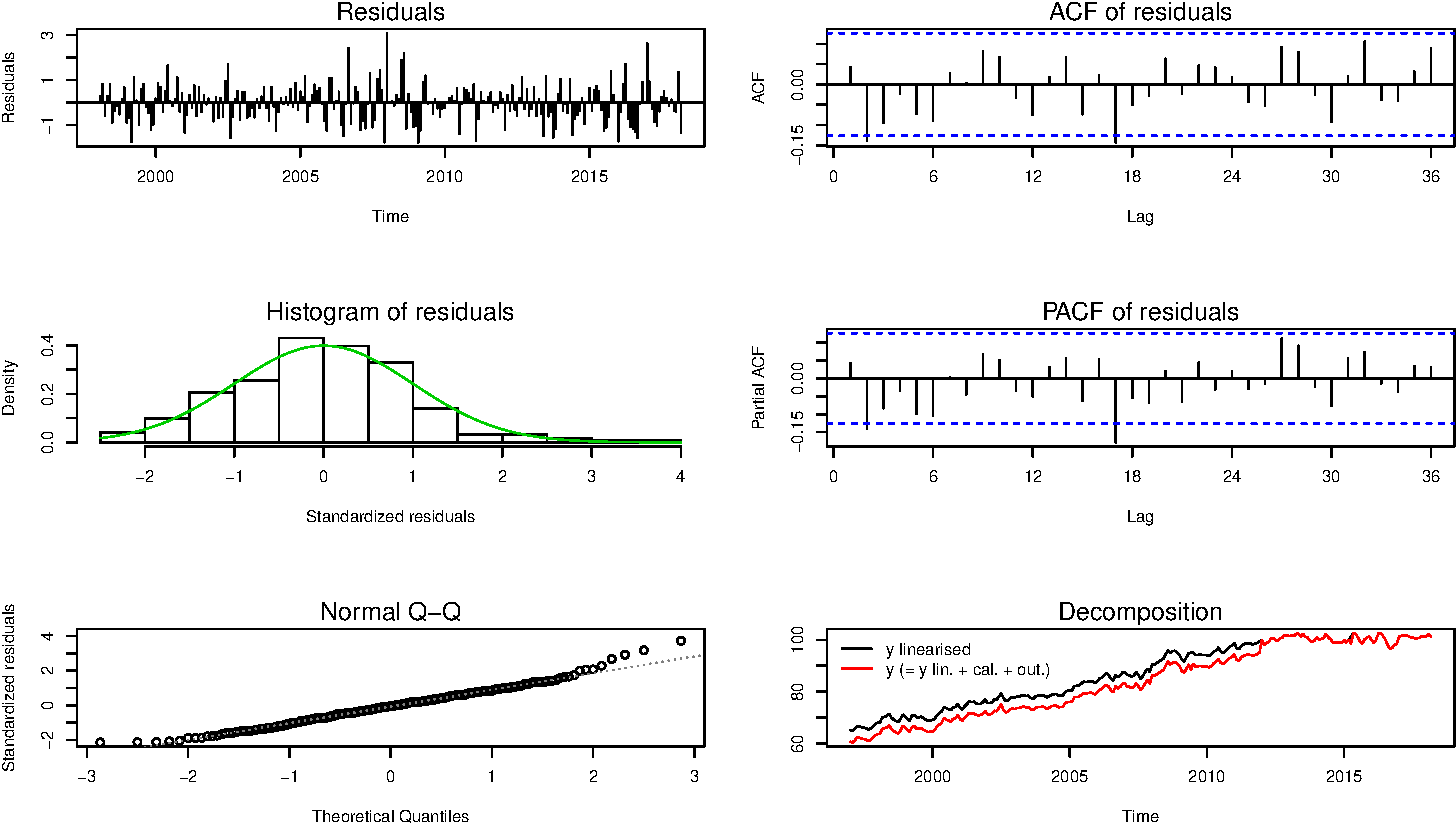
\includegraphics{Diapos/1 - R et JDemetra+_files/figure-beamer/unnamed-chunk-11-1.pdf}

\end{frame}

\begin{frame}[fragile]{RegARIMA : exemples (4/4)}
\protect\hypertarget{regarima-exemples-44}{}

\begin{Shaded}
\begin{Highlighting}[]
\KeywordTok{plot}\NormalTok{(regarima_model, }\DataTypeTok{which =} \DecValTok{7}\NormalTok{)}
\end{Highlighting}
\end{Shaded}

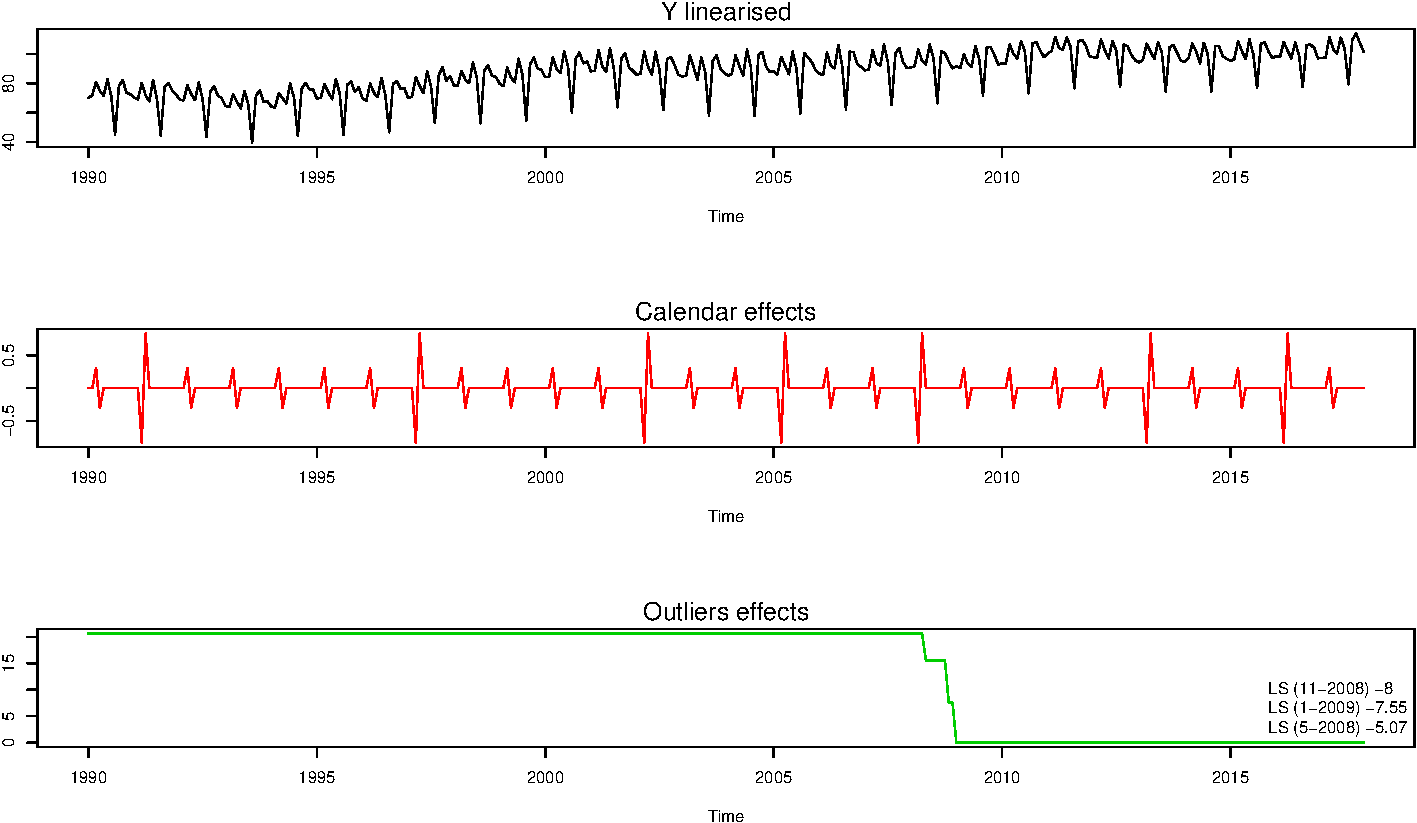
\includegraphics{Diapos/1 - R et JDemetra+_files/figure-beamer/unnamed-chunk-13-1.pdf}

\end{frame}

\hypertarget{cvs-cjo-exemples}{%
\subsection{CVS-CJO : exemples}\label{cvs-cjo-exemples}}

\begin{frame}[fragile]{CVS-CJO : exemples (1/8)}
\protect\hypertarget{cvs-cjo-exemples-18}{}

Un object \texttt{SA} est une \texttt{list()} de 5 éléments:

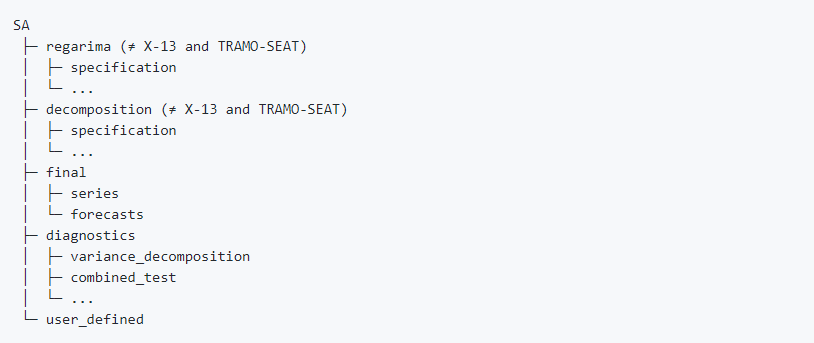
\includegraphics{img/sa_obj_struct.png}

\end{frame}

\begin{frame}[fragile]{CVS-CJO : exemples (2/8)}
\protect\hypertarget{cvs-cjo-exemples-28}{}

Possibilité de définir ses propres spécifications comme sous JD+ ou
d'utiliser les spécifications prédéfinies:

\footnotesize

\begin{Shaded}
\begin{Highlighting}[]
\NormalTok{x13_usr_spec <-}\StringTok{ }\KeywordTok{x13_spec}\NormalTok{(}\DataTypeTok{spec =} \KeywordTok{c}\NormalTok{(}\StringTok{"RSA5c"}\NormalTok{),}
                             \DataTypeTok{usrdef.outliersEnabled =} \OtherTok{TRUE}\NormalTok{,}
                             \DataTypeTok{usrdef.outliersType =} \KeywordTok{c}\NormalTok{(}\StringTok{"LS"}\NormalTok{, }\StringTok{"AO"}\NormalTok{),}
                             \DataTypeTok{usrdef.outliersDate =} \KeywordTok{c}\NormalTok{(}\StringTok{"2008-10-01"}\NormalTok{,}
                                                     \StringTok{"2002-01-01"}\NormalTok{),}
                             \DataTypeTok{usrdef.outliersCoef =} \KeywordTok{c}\NormalTok{(}\DecValTok{36}\NormalTok{, }\DecValTok{14}\NormalTok{),}
                             \DataTypeTok{transform.function =} \StringTok{"None"}\NormalTok{)}
\NormalTok{x13_mod <-}\StringTok{ }\KeywordTok{x13}\NormalTok{(ipch_benin, x13_usr_spec)}
\NormalTok{ts_mod <-}\StringTok{ }\KeywordTok{tramoseats}\NormalTok{(ipch_benin, }\DataTypeTok{spec =} \StringTok{"RSAfull"}\NormalTok{)}
\end{Highlighting}
\end{Shaded}

\end{frame}

\begin{frame}[fragile]{CVS-CJO : exemples (3/8): decomposition}
\protect\hypertarget{cvs-cjo-exemples-38-decomposition}{}

\footnotesize

\begin{Shaded}
\begin{Highlighting}[]
\NormalTok{x13_mod}\OperatorTok{$}\NormalTok{decomposition}
\end{Highlighting}
\end{Shaded}

\begin{verbatim}
##  Monitoring and Quality Assessment Statistics:  
##       M stats
## M(1)    1.817
## M(2)    0.142
## M(3)    0.219
## M(4)    1.600
## M(5)    0.458
## M(6)    0.199
## M(7)    0.786
## M(8)    1.564
## M(9)    0.354
## M(10)   2.682
## M(11)   2.620
## Q       0.905
## Q-M2    1.000
## 
## Final filters: 
## Seasonal filter:  3x5
## Trend filter:  13-Henderson
\end{verbatim}

\end{frame}

\begin{frame}[fragile]{CVS-CJO : exemples (4/8): decomposition}
\protect\hypertarget{cvs-cjo-exemples-48-decomposition}{}

\footnotesize

\begin{Shaded}
\begin{Highlighting}[]
\NormalTok{ts_mod}\OperatorTok{$}\NormalTok{decomposition}
\end{Highlighting}
\end{Shaded}

\begin{verbatim}
## Model
## D :  1 - B - B^12 + B^13 
## MA :  1 - 0.923007 B^12 
## 
## 
## SA
## D :  1 - 2.000000 B + B^2 
## MA :  1 - 0.993616 B + 0.000268 B^2 
## Innovation variance:  0.9301857 
## 
## Trend
## D :  1 - 2.000000 B + B^2 
## MA :  1 + 0.006654 B - 0.993346 B^2 
## Innovation variance:  0.2324235 
## 
## Seasonal
## D :  1 + B + B^2 + B^3 + B^4 + B^5 + B^6 + B^7 + B^8 + B^9 + B^10 + B^11 
## MA :  1 + 1.840644 B + 2.192789 B^2 + 2.271402 B^3 + 2.121758 B^4 + 1.844037 B^5 + 1.499420 B^6 + 1.118113 B^7 + 0.775927 B^8 + 0.431355 B^9 + 0.218509 B^10 - 0.120918 B^11 
## Innovation variance:  0.002063135 
## 
## Irregular
## Innovation variance:  0.2311263
\end{verbatim}

\end{frame}

\begin{frame}[fragile]{CVS-CJO : exemples (5/8)}
\protect\hypertarget{cvs-cjo-exemples-58}{}

\begin{Shaded}
\begin{Highlighting}[]
\KeywordTok{plot}\NormalTok{(x13_mod}\OperatorTok{$}\NormalTok{decomposition)}
\end{Highlighting}
\end{Shaded}

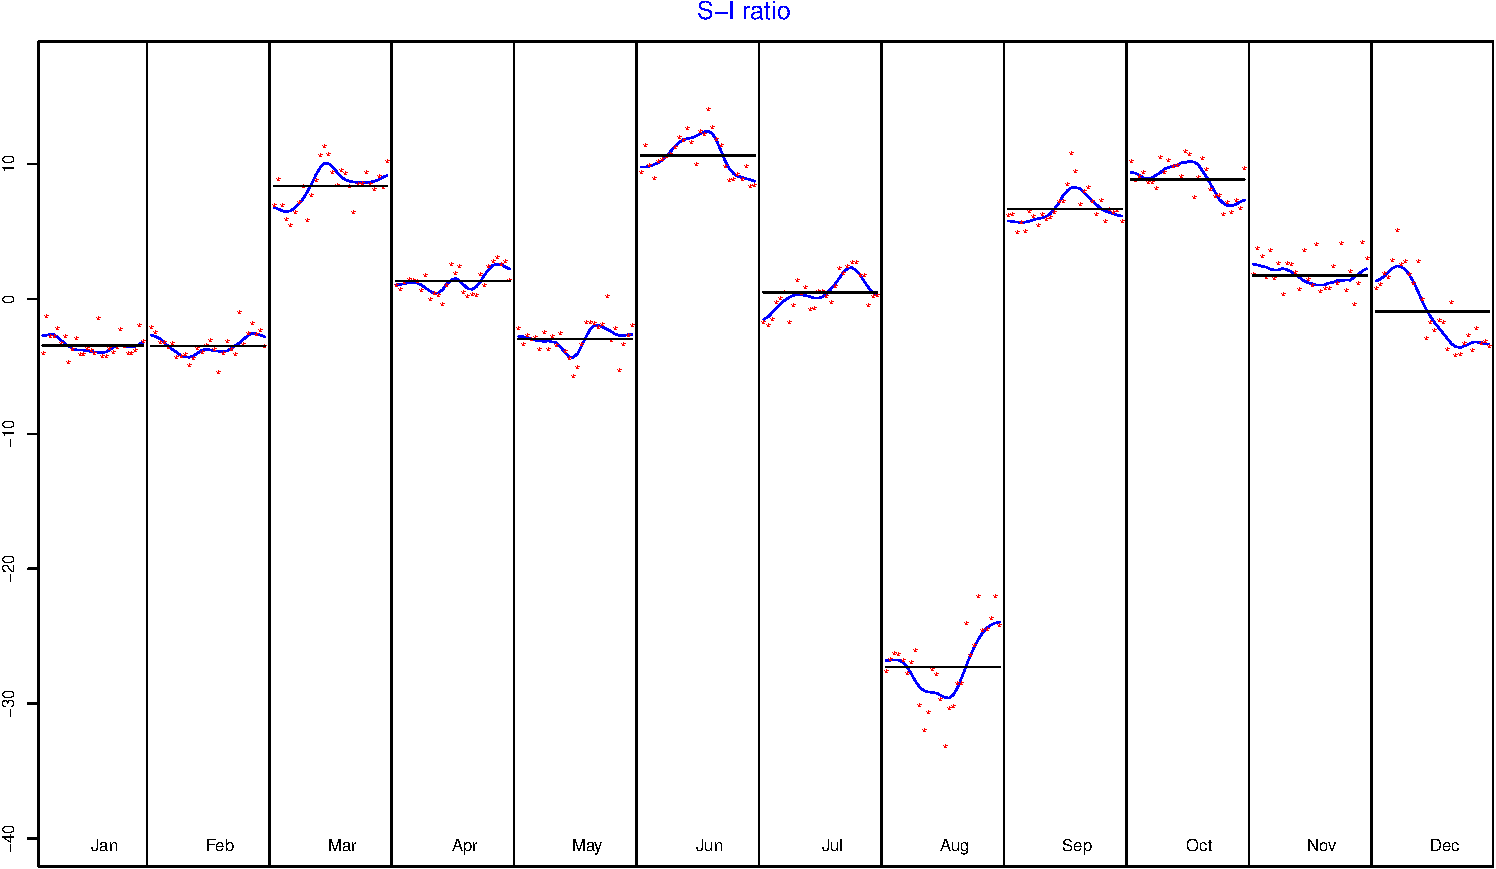
\includegraphics{Diapos/1 - R et JDemetra+_files/figure-beamer/unnamed-chunk-17-1.pdf}

\end{frame}

\begin{frame}[fragile]{CVS-CJO : exemples (6/8)}
\protect\hypertarget{cvs-cjo-exemples-68}{}

\footnotesize

\begin{Shaded}
\begin{Highlighting}[]
\NormalTok{x13_mod}\OperatorTok{$}\NormalTok{final}
\end{Highlighting}
\end{Shaded}

\begin{verbatim}
## Last observed values
##              y        sa        t          s           i
## Apr 2017 101.8 100.85746 100.7578  0.9425435  0.09963373
## May 2017 101.4  99.63078 100.6708  1.7692187 -1.04001487
## Jun 2017 101.0  99.89153 100.6970  1.1084675 -0.80548123
## Jul 2017 100.9 100.64861 100.9250  0.2513894 -0.27642041
## Aug 2017 100.6 101.58999 101.3019 -0.9899894  0.28805653
## Sep 2017 100.6 102.15194 101.6705 -1.5519386  0.48143928
## Oct 2017 100.8 101.99956 101.8910 -1.1995588  0.10858753
## Nov 2017 101.4 101.95044 101.8879 -0.5504364  0.06254215
## Dec 2017 101.3 101.67004 101.6865 -0.3700423 -0.01650179
## Jan 2018 101.3 101.08775 101.3844  0.2122531 -0.29663316
## Feb 2018 102.1 101.97830 101.0979  0.1217027  0.88041793
## Mar 2018 101.2 100.80670 100.9083  0.3933017 -0.10164685
## 
## Forecasts:
##               y_f     sa_f      t_f        s_f          i_f
## Apr 2018 101.8030 100.8442 100.8714  0.9587153 -0.027176702
## May 2018 102.3456 100.6397 101.0182  1.7059430 -0.378560946
## Jun 2018 102.3288 101.2726 101.3284  1.0561489 -0.055725767
## Jul 2018 102.0091 101.7807 101.7358  0.2283849  0.044981509
## Aug 2018 101.2564 102.2454 102.1545 -0.9889700  0.090908471
## Sep 2018 101.1620 102.7472 102.4850 -1.5852315  0.262148762
## Oct 2018 101.4710 102.7393 102.6320 -1.2683186  0.107324026
## Nov 2018 101.9572 102.4970 102.6052 -0.5397680 -0.108215989
## Dec 2018 102.2890 102.6742 102.4825 -0.3852004  0.191679003
## Jan 2019 102.5747 102.3274 102.3341  0.2473195 -0.006675295
## Feb 2019 102.1379 101.9273 102.1834  0.2106156 -0.256118262
## Mar 2019 102.4679 102.0082 102.0327  0.4597346 -0.024581792
\end{verbatim}

\end{frame}

\begin{frame}[fragile]{CVS-CJO : exemples (7/8)}
\protect\hypertarget{cvs-cjo-exemples-78}{}

\begin{Shaded}
\begin{Highlighting}[]
\KeywordTok{plot}\NormalTok{(x13_mod}\OperatorTok{$}\NormalTok{final, }\DataTypeTok{first_date =} \DecValTok{2012}\NormalTok{, }\DataTypeTok{type_chart =} \StringTok{"sa-trend"}\NormalTok{)}
\end{Highlighting}
\end{Shaded}

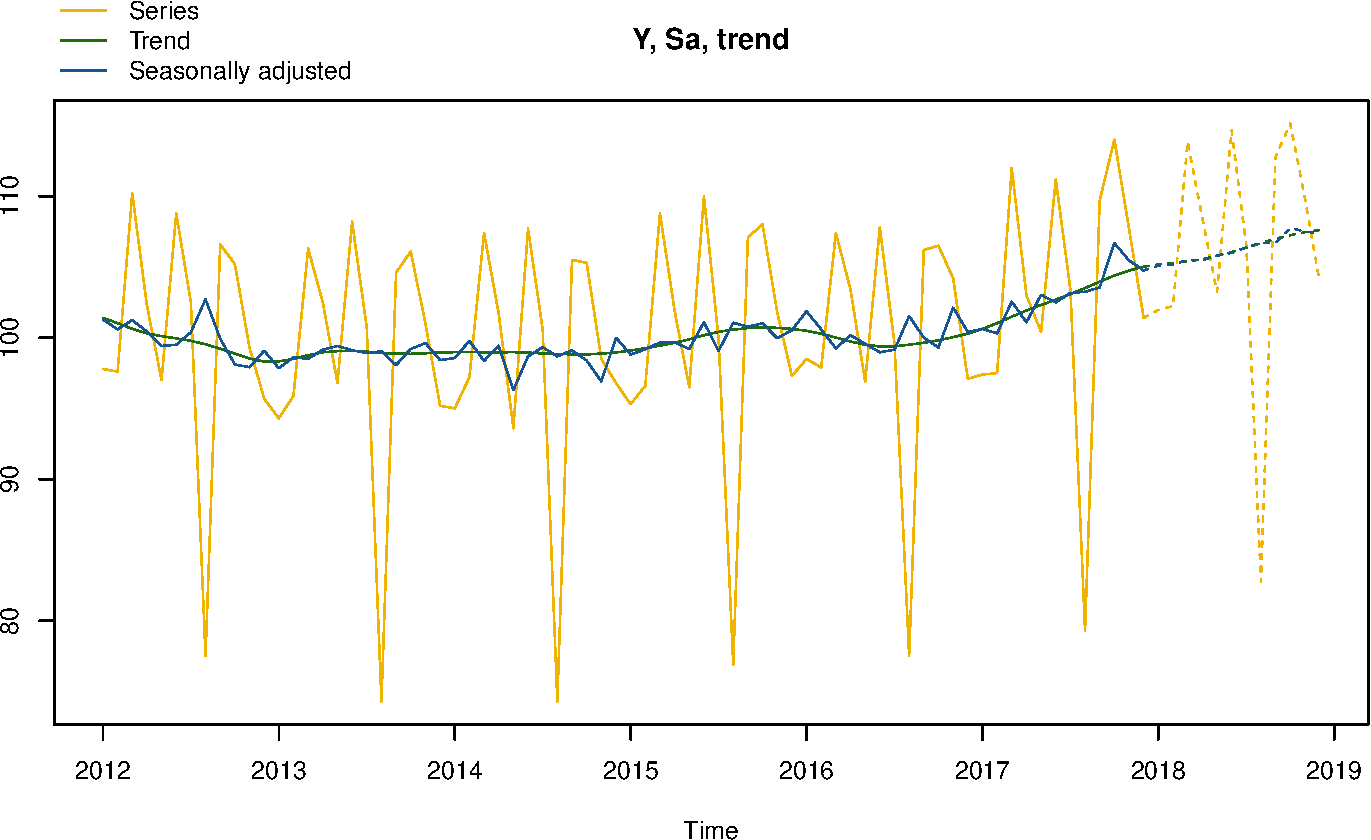
\includegraphics{Diapos/1 - R et JDemetra+_files/figure-beamer/unnamed-chunk-19-1.pdf}

\end{frame}

\begin{frame}[fragile]{CVS-CJO : exemples (8/8)}
\protect\hypertarget{cvs-cjo-exemples-88}{}

\footnotesize

\begin{Shaded}
\begin{Highlighting}[]
\NormalTok{x13_mod}\OperatorTok{$}\NormalTok{diagnostics}
\end{Highlighting}
\end{Shaded}

\begin{verbatim}
##  Relative contribution of the components to the stationary
##  portion of the variance in the original series,
##  after the removal of the long term trend 
##  Trend computed by Hodrick-Prescott filter (cycle length = 8.0 years)
##            Component
##  Cycle        25.022
##  Seasonal      7.085
##  Irregular     4.953
##  TD & Hol.     0.000
##  Others       64.807
##  Total       101.868
## 
##  Combined test in the entire series 
##  Non parametric tests for stable seasonality
##                                                           P.value
##    Kruskall-Wallis test                                          0
##    Test for the presence of seasonality assuming stability       0
##    Evolutive seasonality test                                    0
##  
##  Identifiable seasonality present
## 
##  Residual seasonality tests 
##                                       P.value
##  qs test on sa                          1.000
##  qs test on i                           1.000
##  f-test on sa (seasonal dummies)        0.989
##  f-test on i (seasonal dummies)         0.998
##  Residual seasonality (entire series)   1.000
##  Residual seasonality (last 3 years)    0.997
##  f-test on sa (td)                      0.618
##  f-test on i (td)                       0.657
\end{verbatim}

\end{frame}

\hypertarget{manipuler-des-workspaces}{%
\subsection{Manipuler des workspaces}\label{manipuler-des-workspaces}}

\begin{frame}[fragile]{Exporter un workspace}
\protect\hypertarget{exporter-un-workspace}{}

\footnotesize

\begin{Shaded}
\begin{Highlighting}[]
\NormalTok{wk <-}\StringTok{ }\KeywordTok{new_workspace}\NormalTok{()}
\KeywordTok{new_multiprocessing}\NormalTok{(wk, }\DataTypeTok{name =} \StringTok{"MP-1"}\NormalTok{)}
\KeywordTok{add_sa_item}\NormalTok{(wk, }\DataTypeTok{multiprocessing =} \StringTok{"MP-1"}\NormalTok{,}
            \DataTypeTok{sa_obj =}\NormalTok{ x13_mod, }\DataTypeTok{name =}  \StringTok{"SA with X13 model 1 "}\NormalTok{)}
\KeywordTok{add_sa_item}\NormalTok{(wk, }\DataTypeTok{multiprocessing =}  \StringTok{"MP-1"}\NormalTok{,}
            \DataTypeTok{sa_obj =}\NormalTok{ ts_mod, }\DataTypeTok{name =} \StringTok{"SA with TramoSeats model 1"}\NormalTok{)}
\KeywordTok{save_workspace}\NormalTok{(wk, }\StringTok{"workspace.xml"}\NormalTok{)}
\end{Highlighting}
\end{Shaded}

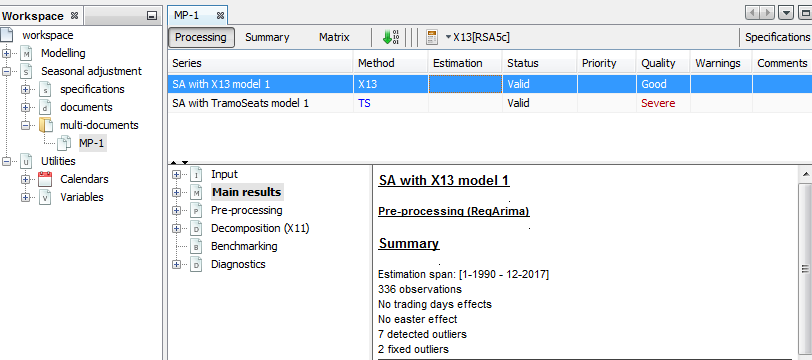
\includegraphics{img/workspace.png}

\end{frame}

\begin{frame}[fragile]{Importer un workspace (1/3)}
\protect\hypertarget{importer-un-workspace-13}{}

\footnotesize

\begin{Shaded}
\begin{Highlighting}[]
\NormalTok{wk <-}\StringTok{ }\KeywordTok{load_workspace}\NormalTok{(}\StringTok{"workspace.xml"}\NormalTok{)}
\KeywordTok{get_ts}\NormalTok{(wk)}
\end{Highlighting}
\end{Shaded}

\begin{verbatim}
## $`MP-1`
## $`MP-1`$`SA with X13 model 1 `
##        Jan   Feb   Mar   Apr   May   Jun   Jul   Aug   Sep   Oct   Nov   Dec
## 1997  60.8  60.5  61.3  62.4  62.3  62.0  61.8  61.5  61.1  61.5  62.4  63.2
## 1998  63.7  63.8  65.7  66.0  66.3  67.1  65.7  64.9  64.3  64.0  65.1  66.8
## 1999  66.1  65.2  64.5  66.5  66.7  65.8  65.7  66.1  65.4  64.9  64.5  64.6
## 2000  64.7  65.3  66.7  67.4  68.1  69.8  69.3  68.9  68.5  69.6  69.7  71.0
## 2001  69.5  68.8  70.0  70.8  71.9  71.6  71.8  71.1  70.9  71.0  71.6  72.6
## 2002  71.3  71.3  71.5  72.7  72.5  73.7  75.1  73.1  72.0  72.3  73.3  73.5
## 2003  73.4  73.7  73.8  74.2  74.3  74.0  74.1  73.2  72.9  73.8  74.1  74.1
## 2004  74.3  74.0  73.4  73.9  74.4  74.6  74.8  74.0  74.1  74.2  75.6  76.0
## 2005  76.1  76.2  77.9  77.9  78.1  78.7  79.5  79.3  79.5  79.7  79.5  78.9
## 2006  79.7  80.7  81.1  81.9  82.7  82.0  80.6  79.9  82.0  81.3  81.8  83.0
## 2007  83.3  82.1  81.9  81.5  81.8  83.3  82.1  80.7  81.7  83.3  84.4  83.2
## 2008  86.2  86.1  86.7  87.2  87.9  88.4  90.1  91.6  90.5  91.2  91.4  90.7
## 2009  89.9  88.0  87.3  88.8  90.4  88.4  90.7  89.7  89.8  89.9  89.8  89.8
## 2010  89.7  89.4  90.0  91.0  91.6  92.6  91.2  90.6  91.2  92.1  93.0  93.4
## 2011  94.3  92.3  92.0  93.2  93.8  94.2  94.3  94.2  93.8  94.1  94.4  95.1
## 2012  99.8  98.1  98.8  99.2 100.5 100.6  99.9  99.6 100.7 100.8 101.9 101.6
## 2013 101.5 101.6 101.4 102.3 102.4 101.3 102.3 101.2 100.9  99.7  99.1  99.7
## 2014 100.9 100.0 100.3 100.6 102.2 101.0 100.2  99.1  98.8  99.2  98.7  99.0
## 2015  99.9  99.0  99.9  98.6 102.5 102.3 100.9  99.2  98.6 100.2 100.9 101.2
## 2016  99.8  98.8 100.0 102.5 102.5 101.5 100.1  98.1  96.5  96.8  98.1  98.4
## 2017 101.2 101.5 101.7 101.8 101.4 101.0 100.9 100.6 100.6 100.8 101.4 101.3
## 2018 101.3 102.1 101.2                                                      
## 
## $`MP-1`$`SA with TramoSeats model 1`
##        Jan   Feb   Mar   Apr   May   Jun   Jul   Aug   Sep   Oct   Nov   Dec
## 1997  60.8  60.5  61.3  62.4  62.3  62.0  61.8  61.5  61.1  61.5  62.4  63.2
## 1998  63.7  63.8  65.7  66.0  66.3  67.1  65.7  64.9  64.3  64.0  65.1  66.8
## 1999  66.1  65.2  64.5  66.5  66.7  65.8  65.7  66.1  65.4  64.9  64.5  64.6
## 2000  64.7  65.3  66.7  67.4  68.1  69.8  69.3  68.9  68.5  69.6  69.7  71.0
## 2001  69.5  68.8  70.0  70.8  71.9  71.6  71.8  71.1  70.9  71.0  71.6  72.6
## 2002  71.3  71.3  71.5  72.7  72.5  73.7  75.1  73.1  72.0  72.3  73.3  73.5
## 2003  73.4  73.7  73.8  74.2  74.3  74.0  74.1  73.2  72.9  73.8  74.1  74.1
## 2004  74.3  74.0  73.4  73.9  74.4  74.6  74.8  74.0  74.1  74.2  75.6  76.0
## 2005  76.1  76.2  77.9  77.9  78.1  78.7  79.5  79.3  79.5  79.7  79.5  78.9
## 2006  79.7  80.7  81.1  81.9  82.7  82.0  80.6  79.9  82.0  81.3  81.8  83.0
## 2007  83.3  82.1  81.9  81.5  81.8  83.3  82.1  80.7  81.7  83.3  84.4  83.2
## 2008  86.2  86.1  86.7  87.2  87.9  88.4  90.1  91.6  90.5  91.2  91.4  90.7
## 2009  89.9  88.0  87.3  88.8  90.4  88.4  90.7  89.7  89.8  89.9  89.8  89.8
## 2010  89.7  89.4  90.0  91.0  91.6  92.6  91.2  90.6  91.2  92.1  93.0  93.4
## 2011  94.3  92.3  92.0  93.2  93.8  94.2  94.3  94.2  93.8  94.1  94.4  95.1
## 2012  99.8  98.1  98.8  99.2 100.5 100.6  99.9  99.6 100.7 100.8 101.9 101.6
## 2013 101.5 101.6 101.4 102.3 102.4 101.3 102.3 101.2 100.9  99.7  99.1  99.7
## 2014 100.9 100.0 100.3 100.6 102.2 101.0 100.2  99.1  98.8  99.2  98.7  99.0
## 2015  99.9  99.0  99.9  98.6 102.5 102.3 100.9  99.2  98.6 100.2 100.9 101.2
## 2016  99.8  98.8 100.0 102.5 102.5 101.5 100.1  98.1  96.5  96.8  98.1  98.4
## 2017 101.2 101.5 101.7 101.8 101.4 101.0 100.9 100.6 100.6 100.8 101.4 101.3
## 2018 101.3 102.1 101.2
\end{verbatim}

\end{frame}

\begin{frame}{Importer un workspace (2/3)}
\protect\hypertarget{importer-un-workspace-23}{}

\animategraphics[loop, autoplay, width=\linewidth]{2.5}{img/gif/import_model/}{1}{114}

\end{frame}

\begin{frame}[fragile]{Importer un workspace (3/3)}
\protect\hypertarget{importer-un-workspace-33}{}

\footnotesize

\begin{Shaded}
\begin{Highlighting}[]
\KeywordTok{compute}\NormalTok{(wk) }\CommentTok{# Important to get the Sa model}
\NormalTok{models <-}\StringTok{ }\KeywordTok{get_model}\NormalTok{(wk) }\CommentTok{# A progress bar is printed by default}
\end{Highlighting}
\end{Shaded}

\begin{verbatim}
## Multiprocessing 1 on 1:
## 
  |                                                                            
  |                                                                      |   0%
  |                                                                            
  |===================================                                   |  50%
  |                                                                            
  |======================================================================| 100%
\end{verbatim}

\begin{Shaded}
\begin{Highlighting}[]
\CommentTok{# To extract only one model}
\NormalTok{mp <-}\StringTok{ }\KeywordTok{get_object}\NormalTok{(wk, }\DecValTok{1}\NormalTok{)}
\KeywordTok{count}\NormalTok{(mp)}
\end{Highlighting}
\end{Shaded}

\begin{verbatim}
## [1] 2
\end{verbatim}

\begin{Shaded}
\begin{Highlighting}[]
\NormalTok{sa2 <-}\StringTok{ }\KeywordTok{get_object}\NormalTok{(mp,}\DecValTok{2}\NormalTok{)}
\KeywordTok{get_name}\NormalTok{(sa2)}
\end{Highlighting}
\end{Shaded}

\begin{verbatim}
## [1] "SA with TramoSeats model 1"
\end{verbatim}

\begin{Shaded}
\begin{Highlighting}[]
\NormalTok{mod <-}\StringTok{ }\KeywordTok{get_model}\NormalTok{(wk, sa2)}
\end{Highlighting}
\end{Shaded}

\begin{verbatim}
## Multiprocessing 1 on 1:
## 
  |                                                                            
  |                                                                      |   0%
  |                                                                            
  |===================================                                   |  50%
  |                                                                            
  |======================================================================| 100%
\end{verbatim}

\end{frame}

\hypertarget{ruxe9duire-le-temps-de-calcul}{%
\subsection{Réduire le temps de
calcul}\label{ruxe9duire-le-temps-de-calcul}}

\begin{frame}[fragile]{En manipulant les objets \faJava{} objects (1/2)}
\protect\hypertarget{en-manipulant-les-objets-objects-12}{}

\footnotesize

Les fonctions de base peuvent être chronophages (calcul de tous les
outpus)\ldots{} Notamment lorsqu'on ne s'intéresse qu'à un seul
paramètre (série désaisonnalisée, tendance, etc.)

\(\rightarrow\) Solution : manipuler les objets Java: \texttt{jx13},
\texttt{jtramoseats}, \texttt{jregarima}, \texttt{jregarima\_x13},
\texttt{jregarima\_tramoseats} and \texttt{get\_jmodel}

\medskip
\pause

\begin{Shaded}
\begin{Highlighting}[]
\NormalTok{jx13_mod <-}\StringTok{ }\KeywordTok{jx13}\NormalTok{(ipch_benin, x13_usr_spec)}
\CommentTok{# To get the available outputs:}
\KeywordTok{tail}\NormalTok{(}\KeywordTok{get_dictionary}\NormalTok{(jx13_mod), }\DecValTok{2}\NormalTok{)}
\end{Highlighting}
\end{Shaded}

\begin{verbatim}
## [1] "diagnostics.msr-global" "diagnostics.msr(*)"
\end{verbatim}

\begin{Shaded}
\begin{Highlighting}[]
\CommentTok{# To get an indicator:}
\KeywordTok{get_indicators}\NormalTok{(jx13_mod, }\StringTok{"diagnostics.ic-ratio"}\NormalTok{)}
\end{Highlighting}
\end{Shaded}

\begin{verbatim}
## $`diagnostics.ic-ratio`
## [1] 2.020626
\end{verbatim}

\begin{Shaded}
\begin{Highlighting}[]
\CommentTok{# To get the previous R output}
\NormalTok{x13_mod <-}\StringTok{ }\KeywordTok{jSA2R}\NormalTok{(jx13_mod)}
\end{Highlighting}
\end{Shaded}

\end{frame}

\begin{frame}{Performance}
\protect\hypertarget{performance}{}

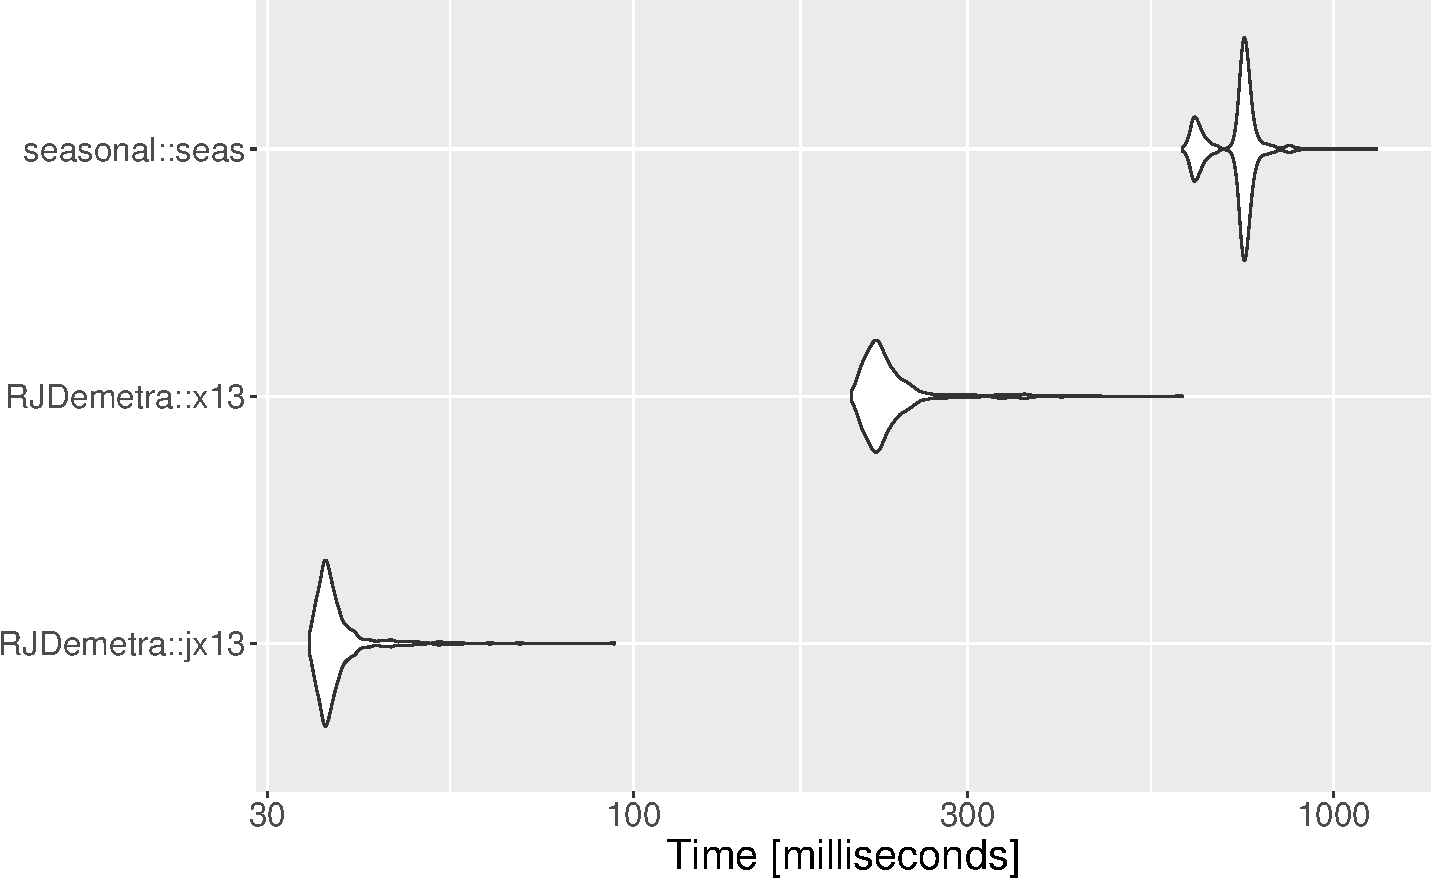
\includegraphics{Diapos/1 - R et JDemetra+_files/figure-beamer/unnamed-chunk-25-1.pdf}

\end{frame}

\hypertarget{autour-de-rjdemetra}{%
\subsection{Autour de RJDemetra}\label{autour-de-rjdemetra}}

\begin{frame}{Exemples d'utilisation de RJDemetra}
\protect\hypertarget{exemples-dutilisation-de-rjdemetra}{}

\begin{itemize}
\tightlist
\item
  rjdqa (sur le CRAN) : package pour aider à évaluer la qualité de la
  désaisonnalisation (tableau de bord et bientôt tests de saisonnalité)
\end{itemize}

\faGithub{} \url{https://github.com/AQLT/rjdqa}

\begin{itemize}
\tightlist
\item
  ggdemetra (sur le CRAN) : intégrer la désaisonnalisation à ggplot2
\end{itemize}

\faGithub{} \url{https://github.com/AQLT/ggdemetra}

\begin{itemize}
\tightlist
\item
  rjdworkspace (en développement) : fonctions supplémentaires pour
  manipuler les workspaces
\end{itemize}

\faGithub{} \url{https://github.com/AQLT/rjdworkspace}

\begin{itemize}
\tightlist
\item
  rjdmarkdown (en développement) : pour exporter directement les modèles
  en PDF/HTML
\end{itemize}

\faGithub{} \url{https://github.com/AQLT/rjdmarkdown}

\begin{itemize}
\tightlist
\item
  Réalisations d'études : Ladiray D., Quartier-la-Tente A., ``Du bon
  usage des modèles Reg-ARIMA en désaisonnalisation'', JMS 2018
\end{itemize}

\end{frame}

\begin{frame}[fragile]{Travaux pratiques \bcoutil}
\protect\hypertarget{travaux-pratiques}{}

Maintenant à vous de jouer !

Documents sous : \url{https://github.com/AQLT/BCEAO_2020}

Objectifs du TP :

\begin{itemize}
\item
  Prendre en main \texttt{rjwsacruncher} et mettre à jour son workspace
\item
  Prendre en main \texttt{RJDemetra} : faire une désaisonnalisation sous
  R, changer la spécification, exporter et importer un workspace.
\end{itemize}

\end{frame}

\end{document}
